\documentclass[12pt]{article}
\title{Part IIA Paper 3 Project}
\author{
	2842A
}

\newcommand\wordcount{
	\immediate\write18{texcount -sum -1 \jobname.tex > count.txt} 
	\input{count.txt}
}

\usepackage[a4paper, total={6.25in, 10in}]{geometry} % to adjust the margins etc
\usepackage{titlesec} % for the title formatting
\usepackage{setspace} % to set line spacing
\usepackage[parfill]{parskip} % remove the paragraph indentation
\usepackage{caption} % used to allow smaller "notes" under graphs/tables besides the main caption
\usepackage{booktabs} % used for the lines under the headers in the tables
\usepackage{multirow} % to allow multiple row option in table formatting
\usepackage{array} % for struts in formatting table
\usepackage{fancyhdr} % for moving page number to the bottom right corner
\usepackage{amsmath} % for multi line equations aligning
\usepackage{bm} % for bolded math symbols (for vectors)
\usepackage{graphicx}

\titleformat*{\section}{\centering \LARGE}
\pagenumbering{arabic} % add page numbers
% next few lines are to get the page numbers to the bottom right
\pagestyle{fancy}
\fancyhf{}
\renewcommand{\headrulewidth}{0pt} %remove the weird top line from fancy
\fancyfoot[R]{\thepage}

% For citation
\usepackage[backend=biber, bibencoding=utf8, style=apa, natbib]{biblatex}
\addbibresource{Vaccine Uptake Project.bib}


\begin{document}
	\maketitle
	\begin{spacing}{1.5} % set 1.5 line spacing
		Q1. Vaccination take-up rates: Inter-State differences in the USA in 2021.
		
		At the end of 2021 the share of the population fully vaccinated against Covid-19 differed widely across US States.
		
		a) Identify and evaluate the main economic and social factors giving rise to this outcome.
		
		b) On the basis of your answer to a), suggest how high vaccination rates might be achieved across the entire United States.
		
		\wordcount words
		\pagebreak
		\section{Introduction}
		By the end of 2021, only 2\% of people wanted a vaccine and had not yet got it (\cite{kff_kff_2022}). Differences in vaccine uptake is hence likely due to to personal choice. Existing research has highlighted correlations in vaccine uptake by factors such as race and party affiliation (\cite{viswanath_individual_2021}). Causal studies have focused on the effect of media consumption (\cite{pinna_cable_2021}), finding that Fox News consumption causally reduces vaccine uptake.
		
		We aim to explain cross-country variation in uptake based on an implicit model of agents forming beliefs on the costs and benefits of vaccination, and then aim to test the impact of financial incentives, to suggest future policy interventions to increase uptake across the US.
		
		\section{Data and Methods}
		\subsection{Data}
		
		\begin{table}
			\caption{Data Sources}
			\begin{minipage}{6.5in}
	\centering
	\def\sym#1{\ifmmode^{#1}\else\(^{#1}\)\fi}
	\def\arraystretch{1.1}
	\small
	\begin{tabular*}{\textwidth}{@{\extracolsep{\fill}}p{0.25\linewidth}p{0.6\linewidth}p{0.15\linewidth}}
		\hline\hline
		Data&Source&Year\\
		\hline
		2020 Election Results&MIT Election Data and Science Lab's Election Returns Dataverse (\cite{mit_election_data_and_science_lab_county_2022})&2020\\
		Religious Affiliation&Public Religion Research Institute 2020 Census of American Religion (\cite{prri_2020_2020})&2020\\
		Racial Distribution&2020 Decennial Redestricting Dataset, maintained by the US Census Bureau ('the Census') (\cite{census_p1_2020})&2020\\
		Age Distribution&County Characteristics Resident Population Estimates, maintained by the Census (\cite{census_county_2019})&2019\\
		Educational attainment&2015-2019 American Community Survey, maintained by the Census (\cite{usda_ers_usda_2019})& Averaged 2015-2019\\
		Poverty rates&As defined by the Census, from the Small Area Income and Poverty Estimates, maintained by the Census (\cite{usda_ers_usda_2019})&2019\\
		Rurality&The 2013 Rural-Urban Continuum Code, which classifies how rural counties are based on their level of urbanization and proximity to metropolitan areas (documented at \citet{usda_ers_usda_2019-1}), from the same source as above&2013\\
		Income and Cost of Living&Median family income and costs of living obtained from the Economic Policy Institutes Family Budget Calculator (\cite{epi_family_2020}). Costs of living measure allows us to correct nominal median family income to \textit{real} income instead.&2020\\
		COVID-19 Cases by 1 December 2020&The CSSE COVID-19 Data Repository maintained by John Hopkins (\cite{cssegis_covid-19_2022}).&2020\\
		County Adjacency&Mapping of every county in the US to every county it borders, obtained from a dataset maintained by the National Bureau of Economic Research (\cite{nber_county_2010}), originating from a dataset maintained by the Census&N/A\\
		\hline\hline
	\end{tabular*}
	\caption*{\footnotesize{Notes: All datasets tagged each county with their Federal Information Processing Standard Publication (FIPS) codes, which was used to merge them together. All US Territories excluded from the dataset as they lack Presidential voting records. All counties in Alaska and Hawaii excluded due to missing data and different reporting standards (many statistics not reported by county, but other organizational units). Utah's data excluded due to spotty county-level COVID-19 case data in 2020. Outside of these states, the following counties still assigned FIPS codes also had missing records: Bedford and Clifton Forge City, as both were merged into other counties and were non-existent by this time period, Dukes, Nantucket and Barnstable Counties in Massachussets, which had missing vaccination records, Ogala Lakota County in North Dakota, a Native American reservation which remains unorganized and generally lacks data, and Yellowstone National Park, which has no resident population. Final dataset of time-invariant characteristics was exactly 3075 counties. Note that, while not all data is available for 2020, and so some are from shortly before, we expect these time invariant characteristics to not dramatically change year-to-year in each county. As explained later, the regressions using these variables do not interpret their coefficients causally given omitted variable bias, but treat them as best linear predictors.}}
\end{minipage}
			\label{table:datasources}
		\end{table}
	
		Regressions were generally done on the county level. Data on vaccination rates across time by county (and by state) were all sourced from the CDC (\cite{cdc_covid-19_2022}). A dataset of time-invariant characteristics of each county was also compiled for 3075 counties in the United States. Data sources and details on excluded counties are reported in Table \ref{table:datasources}.
		
		\subsection{Methods}
		The decision on vaccination can reasonably be broken down into its costs and benefits, and beliefs that agents have about them. We expect that in areas of lower population density, or where COVID would generally spread less quickly, the benefit of vaccination would be lower. As COVID-19's fatality rate rises sharply with age (\cite{levin_assessing_2020}), we would expect more vaccination in counties with more elderly (who benefit more). As beliefs on vaccination's benefits and supposed harms seem to be affected by religious status, race, and political identity, we also expect these variables to be explanatory.
		
		We first run the following regression on the cross-sectional dataset of 3075 counties:
		
		\begin{equation} \label{eq:crosssection}
			\begin{split}
				\textrm{vaccuptake}_i = &\beta_0 + \beta_1 \textrm{repvotes}_i + \beta_2 \textrm{whiteevangelical}_i + \beta_3 \textrm{catholic}_i \\ 
				&+ \beta_4 \textrm{black}_i + \beta_5 \textrm{poverty}_i + \beta_6 ln(\textrm{medincome}_i) + \beta_7 ln(\textrm{col}_i) \\ 
				&+ \beta_8 \textrm{pop60to79}_i + \beta_9 \textrm{above80}_i + \beta_{10} \textrm{fullcollege}_i + \beta_{11} \textrm{casespc}_i \\
				&+\boldsymbol{\delta}\cdot \mathbf{rural}_i + \boldsymbol{\gamma}\cdot \mathbf{state}_i + u_i
			\end{split}
		\end{equation}
		
		Where $\textrm{vaccuptake}_i$ is a measure of vaccine uptake for a county $i$. Definitions for each covariate are listed in Table \ref{table:definition}. The model was estimated for a cross-section of vaccine uptake by county as of 31 December 2021, and also for vaccine uptake as of 1 June 2021, to see if the effects of the covariates on uptake had changed over time. We measured vaccine uptake as the percentage of county residents who had taken at least two doses of the vaccine, and also an alternatively looked at the percentage of county residents who had taken at least one dose of the vaccine, to check similarity of coefficients.
		
		\begin{table}
			\caption{Variable Definitions}
			\begin{minipage}{6.5in}
	\centering
	\def\sym#1{\ifmmode^{#1}\else\(^{#1}\)\fi}
	\def\arraystretch{1}
	\begin{tabular*}{\textwidth}{@{\extracolsep{\fill}}lp{0.35\linewidth}p{0.4\linewidth}}
	\hline\hline
		&Definition&Justification\\
		\hline
		repvotes&Percentage (0-100) of county vote that Donald Trump received in the 2020 election&Aim to measure effect of political affiliation, which affects news consumption and beliefs on the costs and benefits of vaccination\\
		whiteevangelical&Percentage (0-100) of county identifying as White Evangelical Protestants as of 2020&Aim to measure effect of religion - White Evangelicals are a heavily conservative and Republican-supporting religious group. (CITE)\\
		catholic&Percentage (0-100) of county identifying as Catholics as of 202&Aim to measure the effect of religion - the Pope has actively extolled the benefits of vaccination (CITE), check effect.\\
		black&Percentage (0-100) of county who are African-American as of 2020&Due to historical grievances and mistrust of government, African-Americans are known to be less likely to choose to vaccinate. (CITE)\\
		poverty&Percentage (0-100) of county under the poverty line as of 2019(as defined by the Census)&Those in poverty may have difficulty finding access to vaccines, or more broadly, access to good-quality information on their costs and benefits.\\
		medincome&Nominal median family income for a family of four, as of 2020&Same reason as above. Poverty variable lets us see if effect is stronger at the low end of the income distribution.\\
		col&Cost of living as of 2020, as measured by the EPI.&Allows coefficient on medincome to be interpreted as the effect of changes in real median income (holding prices/cost of living fixed)\\
		pop60to79&Percentage (0-100) of county aged between 60 and 79 in 2019.&Elderly are at greater risk of death and serious illness from COVID-19\\
		above80&Percentage (0-100) of county aged 80 and above in 2019&See above\\
		fullcollege&Percentage (0-100) of county who completed at least 4 years of college, averaged 2015-2019&Those with college degrees may be less susceptible to misinformation on the supposed harms of vaccination\\
		casespc&Total recorded COVID-19 cases as of 1 December 2020, before the start of the vaccination program.&A proxy for how amenable the area is to COVID-19 spread, which would increase the benefit of vaccination against COVID-19\\
		$\mathbf{rural}$&Vector of dummy variables for each possible score on the 2013 Rural-Urban Continuum Code&More rural areas typically have lower population density and hence less risk of catching COVID-19, and so there are lower benefits to vaccination.\\
		$\mathbf{state}$&Vector of state fixed effects&Allows for variation in state policy responses that affected COVID-19 vaccination rates\\
	\hline\hline
	\end{tabular*}
\end{minipage}

			\label{table:definition}
		\end{table}
	
		As different covariates have different units and standard deviations, interpreting their relative effect sizes (which variables are "more important" in explaining variation in vaccine uptake) can be difficult. Hence we estimated the \textit{beta coefficients} of the model. These are calculated by using the z-score of every variable (defined for a covariate $x_j$, with a sample standard deviation $\hat{\sigma}_j$, as $z_j := \frac{x_{ij}-\bar{x}_j}{\hat{\sigma}_j}$)) and noticing then that, if Model (\ref{eq:crosssection}) holds, then it is also true that
		\begin{equation} \label{eq:standardized}
			z_y=\frac{y_i-\bar{y}}{\hat{\sigma}_y} = \sum_{j=1}^{k} \frac{\hat{\sigma}_j}{\hat{\sigma}_y}\beta_j z_{ij}
		\end{equation}
		
		Hence, we can calculate, for each covariate $x_j$, a beta coefficient $\hat{b}_j := \frac{\hat{\sigma}_j}{\hat{\sigma}_y}\beta_j$, interpreted as the standard deviation change in in $y_i=\textrm{vaccuptake}_i$ from a one standard deviation change in covariate $x_j$. This standardizes the units across the covariates and makes their corresponding effect sizes more directly comparable (although, not perfectly so, as some covariates are drawn from more-spread-out distributions).
		
		We also more explicitly estimate any trends in the covariates over time, by estimating the model:
		
		\begin{equation}
			\textrm{vaccuptake}_{it} =  \beta_0 + \boldsymbol{\alpha}\cdot\mathbf{x}_{i} + \boldsymbol{\beta}\cdot\mathbf{x}_{i}\cdot t + \boldsymbol{\gamma}\cdot\mathbf{x}_{i}\cdot t^2 + u_i
		\end{equation}
		on a panel dataset of observations of vaccine uptake at the start of every month (from May 2021 to March 2021), where $\mathbf{x}_{i}$ is a vector of covariates (including the state fixed effects), using clustered standard errors by county, so as to correct for serial correlation across time in each county. For any covariate $x_j$, we have that
		\begin{equation} \label{eq:trends}
			\frac{\partial \textrm{vaccineuptake}_{it}}{\partial x_{ij}} = \alpha_j + \beta_jt + \gamma_jt^2
		\end{equation}
		Hence, $\beta_j$ and $\gamma_j$ measure a quadratic trend in the effect-size of the covariate on vaccine uptake over time.
		
		
		We cannot interpret any of the coefficients estimated above as estimates of the \textit{causal impact} of the covariates on vaccine uptake. That would assume exogeneity (and strict exogeneity in the panel Model (\ref{eq:trends})), which is unlikely to be satisfied; for example, we cannot conclude, if the coefficient on $ln(\textrm{medincome})$ is positive, that increasing incomes would increase vaccine uptake. Higher incomes may simply correlate with being more informed, an unobserved variable, and so being less susceptible to vaccine misinformations. This would lead to omitted variable bias, biasing the coefficient on $ln(\textrm{medincome})$ upwards. Coefficients simply reflect correlations in the data, which are at best suggestive.
		
		To answer part (b), however, we need to find out what \textit{causes} vaccine uptake to increase. We hence turn our attention to a policy many states attempted in 2021: vaccine lotteries. We will focus in particular on Colorado's "Colorado Comeback Cash" program, where all those who had received at least one dose of the vaccine were eligible for a weekly \$1 million dollar lottery (\cite{murphy_colorado_2021}). The program began on May 25, and ran to June 30 (\cite{thirumurthy_association_2022}).
		
		\begin{figure}
			\centering
			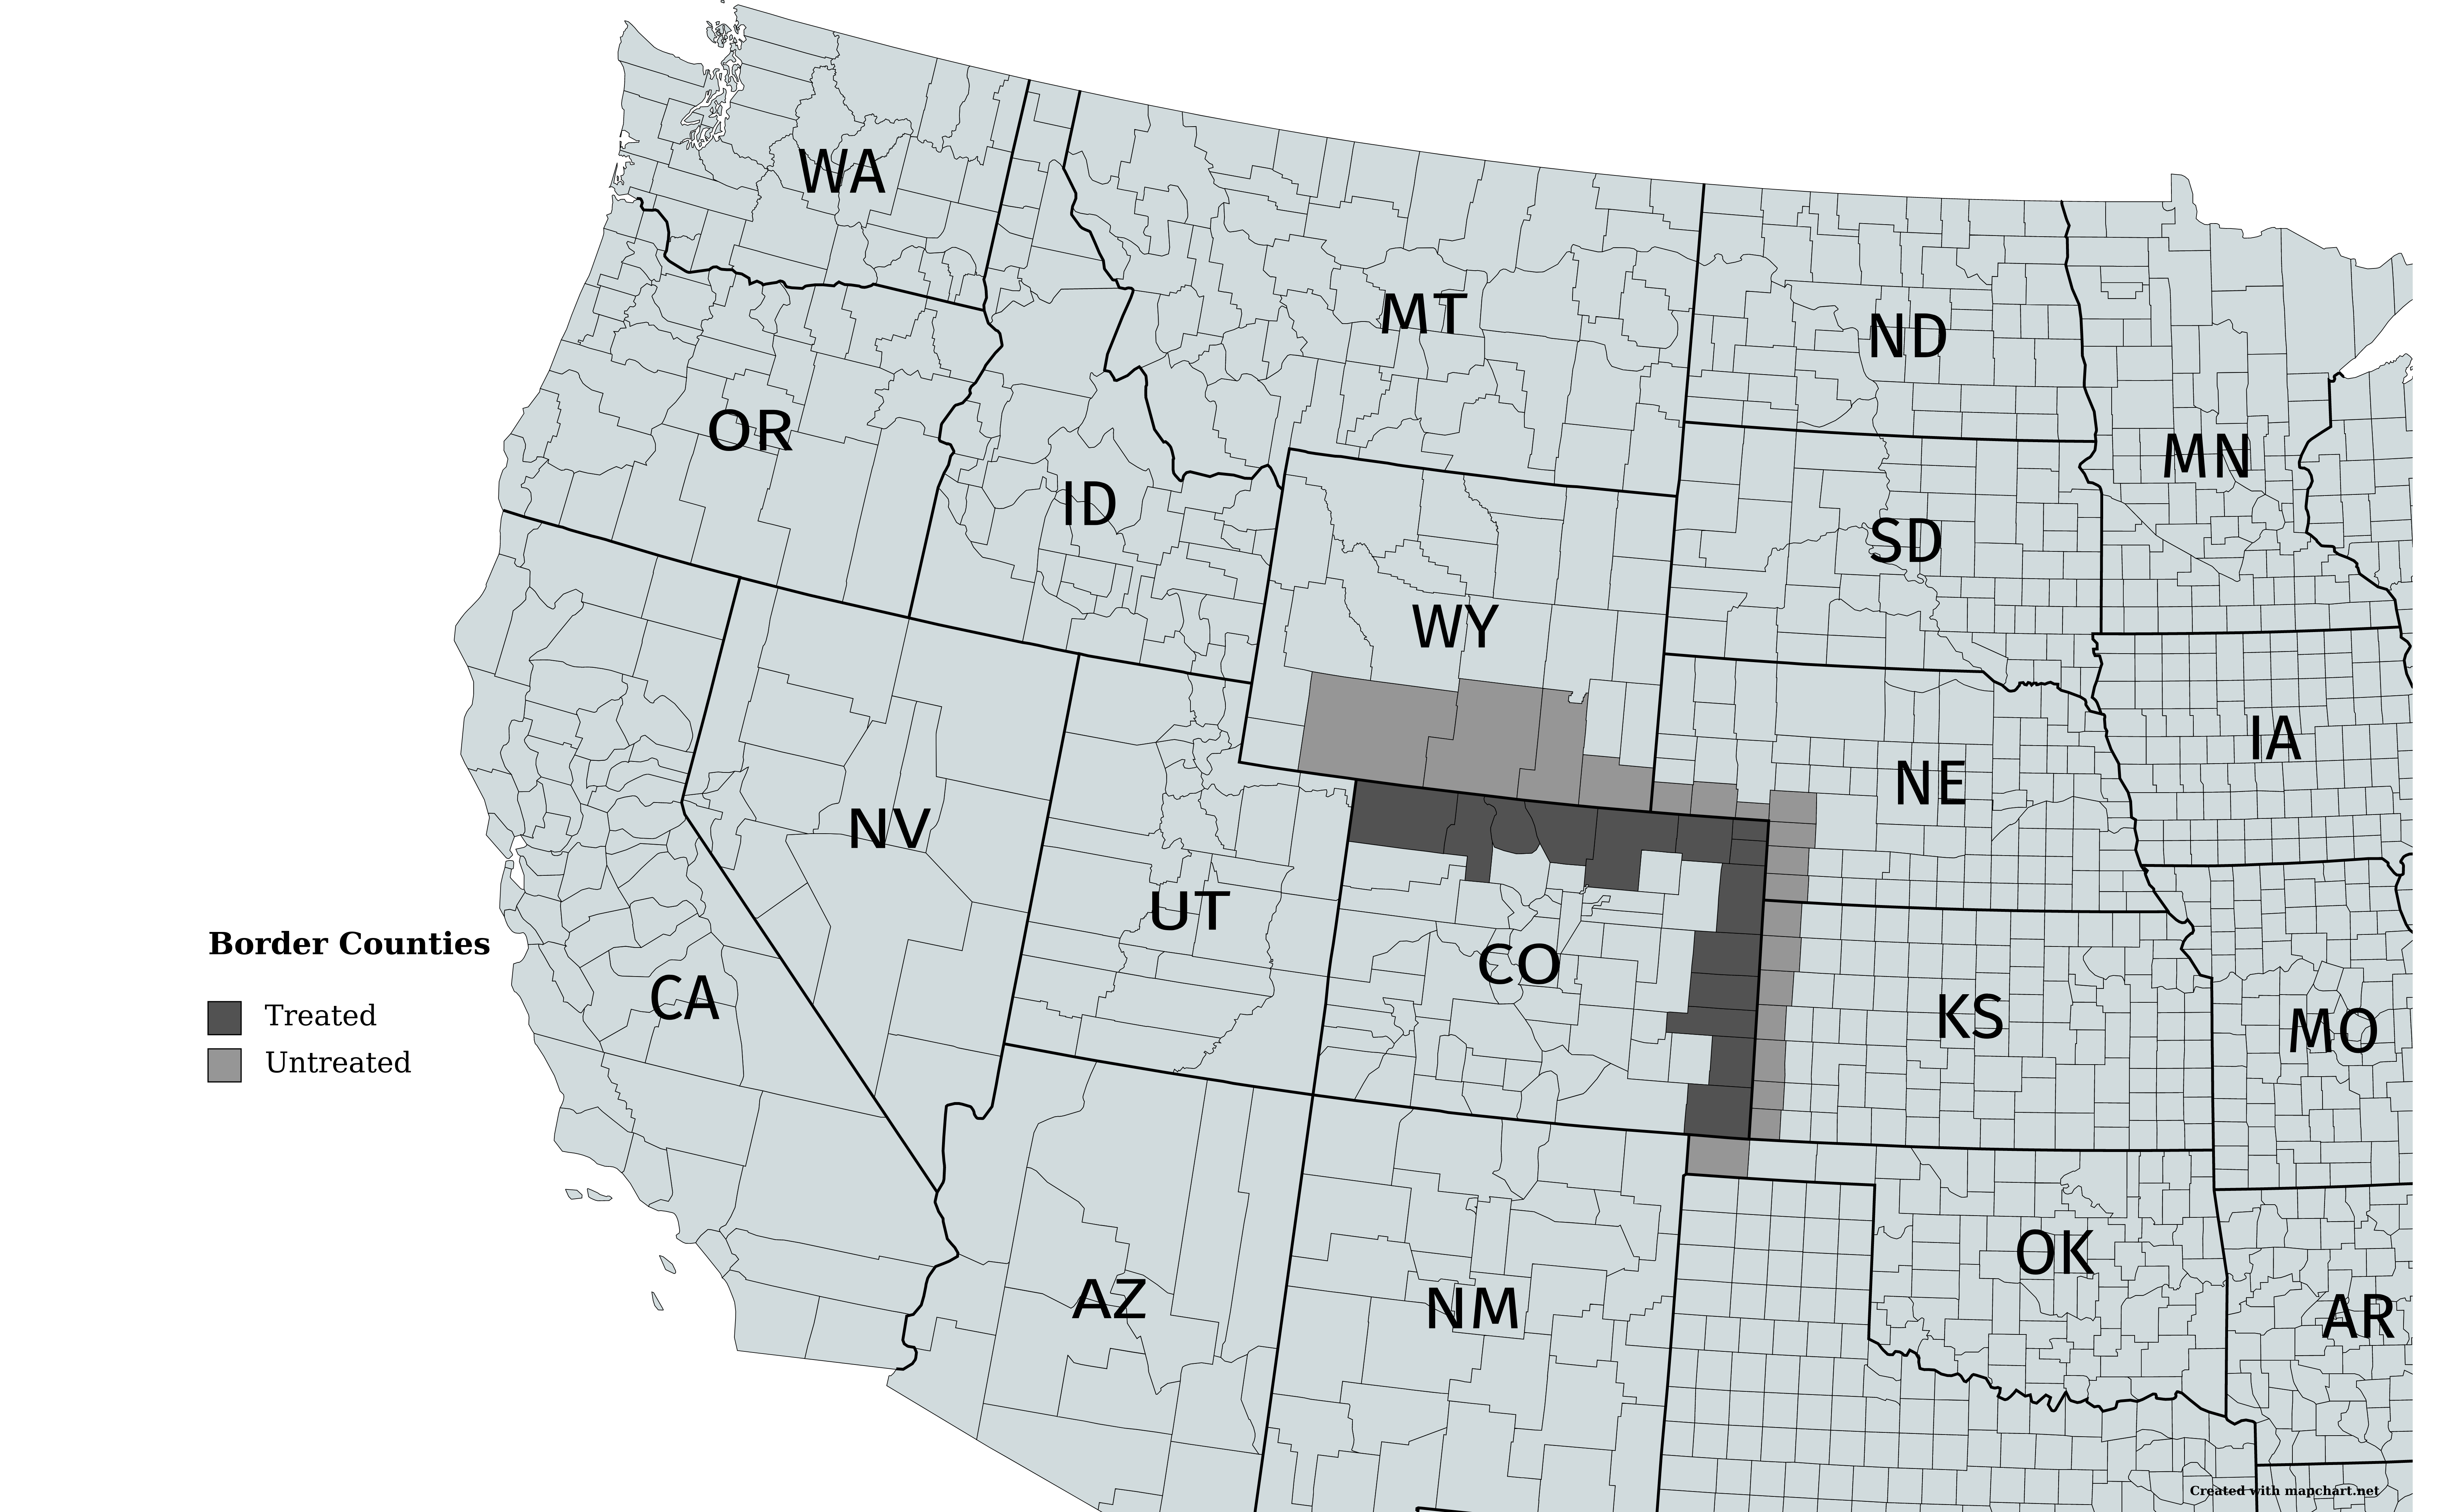
\includegraphics[width=6in]{../graphs/Border_Counties.png}
			\caption*{\footnotesize{Oklahoma, Kansas, Nebraska and Wyoming did not have vaccine lotteries over this period (CITE). New Mexico did, and hence counties bordering New Mexico are excluded from this regression. Utah is excluded from the dataset due to missing data on some covariates. Each county-pair in the pair design dataset consists of one county in Colorado (in dark grey), and one county in an untreated state (in light grey). County-pairs were matched using the NBER county adjacency dataset.}}
			\caption{Counties in Pair Design}
			\label{fig:bordercounties}
		\end{figure}
		
		To evaluate the effect of the vaccine lottery, we use a design inspired by \citet{dube_minimum_2010}. We pick counties in Colorado which border counties in states which did not have vaccine lotteries across this period (see Figure \ref{fig:bordercounties}). We reason that these counties are similar to counties they share a border with - most things which affect one county in any period $t$ will probably also affect a paired county across the state border. Table \ref{table:didsummary} compares the selected border counties on some selected covariates; within each county-pair, differences in covariate values are generally within one standard deviation of the covariate.
		
		\begin{table}
			\centering
			\caption{Summary Statistics}
			\centerline{\begin{minipage}{6.25in}
	\centering
	\def\sym#1{\ifmmode^{#1}\else\(^{#1}\)\fi}
	\def\arraystretch{1.1}
	\begin{tabular}{l*{4}{cc}}
	\hline\hline
	            &\multicolumn{1}{c}{(1)}&\multicolumn{1}{c}{(2)}&\multicolumn{1}{c}{(3)}&\multicolumn{1}{c}{(4)}\\
	            &     Treated&   Untreated&Pair Differences&Nationwide SD\\
	\hline
	repvotes&       72.87&       80.46&        8.65&       16.03\\
	black       &        0.82&        0.72&        0.67&       14.79\\
	fullcollege &       24.75&       24.51&        7.12&        9.54\\
	casespc&        0.04&        0.06&        0.03&        0.02\\
	whiteevangelical&       31.79&       32.67&        6.65&       12.64\\
	catholic    &       13.79&       15.89&        4.45&       10.03\\
	poverty     &       12.81&       11.74&        3.13&        5.78\\
	medinc&    68923.79&    69379.73&    11087.17&    16720.16\\
	pop60to79   &       21.72&       21.87&        3.61&        4.58\\
	above80     &        5.37&        5.98&        1.75&        1.50\\
	\hline
	\(N\)       &          14&          18&          62&        3075\\
	\hline\hline
	\end{tabular}
	\caption*{\footnotesize{Columns 1 and 2 report the average value of the predictive covariates in the treated and untreated groups, corresponding to the Colorado border counties and their neighbors respectively (see Figure \ref{fig:bordercounties}). Column 3 contains the average absolute difference in covariates between two counties along the Colorado border which are connected. Column 4 is the standard deviation of the covariates across the entire nationwide dataset. Covariates are selected as those with the largest standardized effect sizes in Table \ref{table:crosssection}.}}
\end{minipage}
}
			\label{table:didsummary}
		\end{table}
		
		However, only one member of each pair (the county within Colorado) is affected by the lottery. We can hence use the paired non-treated county as a control to estimate the causal impact of the vaccine lottery. We construct a panel of consisting of every cross-border county-pair, from 10 days before the start of the lottery, to 10 days after. We then estimate the model:
		
		\begin{equation} \label{eq:pairdesign}
			\textrm{vaccuptake}_{ipt} = \alpha + \beta \textrm{treated}_{it} + \phi_i + \tau_{pt} + u_{ipt}
		\end{equation}
		
		$i$ is a specific county, $p$ is a county-pair it belongs to, and $t$ is the day in the panel. $\tau_{pt}$ is a pair-specific time fixed effect (shocks beside the lottery happen to both members of a pair) , and $\phi_i$ is a county fixed account (accounting for initial differences). $\textrm{treated}_{it}=1$ if the county $i$ is in Colorado, and $t$ is after 25 May. $\beta$, the effect of the vaccine lottery on vaccine uptake, is consistently estimated if $Cov(\textrm{treated}_{it}, u_{itp})=0$ - ie, if no shocks systematically occured to Colorado counties without affecting the paired counties, after 25 May. We also estimate an alternative model including a $\gamma t\cdot\textrm{treated}_{it}$ term, allowing the effect of the vaccine lottery to change linearly with time over the 10 days post-treatment.
		
		Finally, to further check the robustness of this causal estimate, we utilize a Synthetic Control design, as detailed in (\cite{abadie_using_2021}) and used in prior studies on Ohio's vaccine lottery (\cite{lang_did_2022}). We collapse our 3075 county level dataset into a state-level dataset, and exclude the 23 other states who had vaccine lotteries in this period (\cite{thirumurthy_association_2022}). We construct a synthetic Colorado by taking a weighted average of other states to closely match Colorado on some predictive covariates (we use the results of estimating Model (\ref{eq:standardized}) to gauge which covariates are most important in explaining variation in vaccine uptake). We use these weights to see how vaccine uptake would have evolved in the synthetic Colorado (made of untreated states), and take the difference between the synthetic Colorado and the real Colorado's vaccine uptake on day $t$ as the causal impact of the vaccine lottery on day $t$, and test its significance.
		
		\section{Results and Discussion}
		
		\begin{table}
			\centering
			\caption{Cross-Section Regression}
			\centerline{\begin{minipage}{6.5in}
	\centering
	\def\sym#1{\ifmmode^{#1}\else\(^{#1}\)\fi}
	\def\arraystretch{1.1}
	\begin{tabular*}{\textwidth}{@{\extracolsep{\fill}}l*{5}{cc}}
	\hline\hline
				&\multicolumn{3}{c}{December 31 Sample}     & \multicolumn{2}{c}{June 2 Sample}\\
				\cmidrule{2-4}\cmidrule(l{1ex}r{1ex}){5-6}
	            &\multicolumn{1}{c}{(1)}         &\multicolumn{1}{c}{(2)}&\multicolumn{1}{c}{(3)}         &\multicolumn{1}{c}{(4)}         &\multicolumn{1}{c}{(5)}\\
	            &        \multirow{2}{*}{Two Doses}        &    Two Doses    &       \multirow{2}{*}{One Dose}         &        \multirow{2}{*}{Two Doses}         &        Two Doses\\
	            &&Standardized&&&Standardized\\ 
	\hline
	\multirow{2}{*}{repvotes}&       -0.52\sym{***}&       -0.65&       -0.60\sym{***}&       -0.31\sym{***}&       -0.35\\
	            &      (0.03)         &            &      (0.04)         &      (0.03)         &            \\
	\multirow{2}{*}{whiteevangelical}&       -0.03         &       -0.03&       -0.05         &       -0.04         &       -0.03\\
	            &      (0.06)         &            &      (0.07)         &      (0.05)         &            \\
	\multirow{2}{*}{catholic}    &        0.11\sym{*}  &        0.09&        0.14\sym{**} &       -0.02         &       -0.02\\
	            &      (0.04)         &            &      (0.05)         &      (0.04)         &            \\
	\multirow{2}{*}{black}       &       -0.25\sym{***}&       -0.29&       -0.27\sym{***}&       -0.16\sym{***}&       -0.17\\
	            &      (0.03)         &            &      (0.04)         &      (0.03)         &            \\
	\multirow{2}{*}{poverty}     &       -0.15         &       -0.07&       -0.14         &       -0.13\sym{*}  &       -0.05\\
	            &      (0.08)         &            &      (0.10)         &      (0.06)         &            \\
	\multirow{2}{*}{lmedincome}  &        2.22         &        0.04&        1.33         &        4.01         &        0.07\\
	            &      (2.96)         &            &      (3.46)         &      (2.28)         &            \\
	\multirow{2}{*}{lcol}        &        4.19         &        0.04&        6.37         &        0.41         &        0.00\\
	            &      (3.41)         &            &      (4.19)         &      (3.01)         &            \\
	\multirow{2}{*}{pop60to79}   &        0.18\sym{*}  &        0.06&        0.20\sym{*}  &        0.31\sym{***}&        0.10\\
	            &      (0.08)         &            &      (0.10)         &      (0.06)         &            \\
	\multirow{2}{*}{above80}     &        0.73\sym{***}&        0.08&        0.43         &        0.53\sym{**} &        0.06\\
	            &      (0.21)         &            &      (0.26)         &      (0.17)         &            \\
	\multirow{2}{*}{fullcollege} &        0.10\sym{*}  &        0.07&        0.11\sym{*}  &        0.11\sym{***}&        0.08\\
	            &      (0.04)         &            &      (0.05)         &      (0.03)         &            \\
	\multirow{2}{*}{casespc}&       57.27\sym{***}&        0.11&       55.28\sym{**} &       52.05\sym{**} &        0.09\\
	            &     (15.05)         &            &     (16.87)         &     (16.25)         &            \\
	Constant      &        2.87         &            &        4.21         &      -11.61         &            \\
	            &     (41.54)         &            &     (50.46)         &     (33.07)         &            \\
	rural Wald Statistic&0.72&&1.59&1.08&\\
	\hline
	\(N\)       &        3075         &        3075&        3075         &        3075         &        3075\\
	White Test F-Stat&1.274&&52.24\sym{***}&5.16\sym{**}&\\
	\hline\hline
	\end{tabular*}
	\caption*{\footnotesize{Notes:\\ 
	\sym{*} \(p<0.05\), \sym{**} \(p<0.01\), \sym{***} \(p<0.001\)}}
\end{minipage}
}
			\label{table:crosssection}
		\end{table}
		
		Results from the estimation of Model (\ref{eq:crosssection}) are presented in Table \ref{table:crosssection}. Our estimates (not to be interpreted causally, but reflecting correlations within the data) match prior work and have the expected sign - Republicans and black individuals are less likely to get vaccinated, and this is reflected on the county level. Counties with older people, or more college graduates, are more likely to get vaccinated. Poverty and income have the expected signs, and are jointly significant (see caption), although individually insignificant likely due to multicollinearity. Places which had more cases per person in 2020 had higher vaccination rates in 2021, as hypothesized that the benefits of vaccination would be higher and more clear when this was true.
		
		By comparing beta coefficients, we can identify that by far the factor associated with the biggest effect size on vaccine uptake is the republican vote share in the 2020 election, followed by the number of blacks. These effect sizes seem to grow over time, possibly suggesting an increasing hardening of attitudes towards the vaccine.
		
		\begin{table}
			\centering
			\caption{Coefficient Change Over Time}
			{
\def\sym#1{\ifmmode^{#1}\else\(^{#1}\)\fi}
\begin{tabular}{l*{2}{c}}
\hline\hline
            &\multicolumn{1}{c}{(1)}&\multicolumn{1}{c}{(2)}\\
            &\multicolumn{1}{c}{fullvaxpct}&\multicolumn{1}{c}{fullvaxpct}\\
\hline
c.t c.repvotes2020pct&     -0.0323\sym{***}&     -0.0489\sym{***}\\
            &   (0.00321)         &   (0.00558)         \\
[1em]
c.t c.whiteevangelical&     0.00238         &      0.0148         \\
            &   (0.00515)         &   (0.00792)         \\
[1em]
c. c.catholic&      0.0198\sym{***}&      0.0131\sym{*}  \\
            &   (0.00415)         &   (0.00651)         \\
[1em]
c.t c.black &     -0.0112\sym{***}&    -0.00437         \\
            &   (0.00266)         &   (0.00460)         \\
[1em]
c.t c.poverty&    -0.00860         &     -0.0691\sym{***}\\
            &   (0.00704)         &    (0.0118)         \\
[1em]
c.t c.lmedincome&      -0.223         &      -1.213\sym{**} \\
            &     (0.277)         &     (0.401)         \\
[1em]
c.t c.lcol  &       1.087\sym{***}&       2.204\sym{***}\\
            &     (0.238)         &     (0.466)         \\
[1em]
c.t c.pop60to79&     -0.0158\sym{*}  &     -0.0426\sym{***}\\
            &   (0.00664)         &    (0.0115)         \\
[1em]
c.t c.above80&      0.0135         &    -0.00855         \\
            &    (0.0190)         &    (0.0300)         \\
[1em]
c.t c.fullcollege&    -0.00415         &      0.0173\sym{**} \\
            &   (0.00414)         &   (0.00643)         \\
[1em]
c.t c.cases\_per\_capita&       0.417         &       3.850\sym{*}  \\
            &     (1.271)         &     (1.787)         \\
[1em]
c.t2 c.repvotes2020pct&                     &     0.00139\sym{**} \\
            &                     &  (0.000496)         \\
[1em]
c.t2 c.whiteevangelical&                     &    -0.00104         \\
            &                     &  (0.000745)         \\
[1em]
c.t2 c.catholic&                     &    0.000559         \\
            &                     &  (0.000658)         \\
[1em]
c.t2 c.black&                     &   -0.000566         \\
            &                     &  (0.000459)         \\
[1em]
c.t2 c.poverty&                     &     0.00504\sym{***}\\
            &                     &   (0.00108)         \\
[1em]
c.t2 c.lmedincome&                     &      0.0825\sym{*}  \\
            &                     &    (0.0413)         \\
[1em]
c.t2 c.lcol &                     &     -0.0931\sym{*}  \\
            &                     &    (0.0398)         \\
[1em]
c.t2 c.pop60to79&                     &     0.00224\sym{*}  \\
            &                     &  (0.000975)         \\
[1em]
c.t2 c.above80&                     &     0.00183         \\
            &                     &   (0.00274)         \\
[1em]
c.t2 c.fullcollege&                     &    -0.00179\sym{**} \\
            &                     &  (0.000605)         \\
[1em]
c.t2 c.cases\_per\_capita&                     &      -0.286         \\
            &                     &     (0.156)         \\
\hline
\(N\)       &       33825         &       33825         \\
\hline\hline
\multicolumn{3}{l}{\footnotesize Standard errors in parentheses}\\
\multicolumn{3}{l}{\footnotesize \sym{*} \(p<0.05\), \sym{**} \(p<0.01\), \sym{***} \(p<0.001\)}\\
\end{tabular}
}

			\label{table:trends}
		\end{table}
		
		Catholicism was not associated with higher vaccination rates in June, but was by December. The estimation of Model (\ref{eq:trends}), presented in Table \ref{table:trends} affirms this, as in either specification there is an increase in the effect size of Catholicism over time. While we do not have an adequate design to demonstrate this, this may suggest that the Pope's messaging on vaccination (see \citet{gawel_effects_2021}) has successfully changed attitudes over time. This suggests one way to achieve high vaccination rates across the Untied States: engaging local religious leaders to get them to urge their worshippers to get vaccinated, and to educate them against COVID-19 vaccine related misinformation.
		
		Table \ref{table:trends} also affirms that the Republican and black aversion to vaccination is only getting stronger with time (although, at a declining rate for Republicans, by the coefficient on $t^2\cdot \textrm{repvotes}$). This is again suggestive of polarization, and further highlights the need to break into the Republican and black social networks with pro-vaccine messaging.
		
		\begin{table}
			\centering
			\caption{Effect of Colorado Vaccine Lottery}
			\centerline{\begin{minipage}{6.25in}
	\centering
	\def\sym#1{\ifmmode^{#1}\else\(^{#1}\)\fi}
	\begin{tabular*}{\textwidth}{@{\extracolsep{\fill}} l*{4}{c}}
	\hline\hline
	            &\multicolumn{1}{c}{(1)}&\multicolumn{1}{c}{(2)}&\multicolumn{1}{c}{(3)}&\multicolumn{1}{c}{(4)}\\
	            &\multicolumn{1}{c}{Two Doses}&\multicolumn{1}{c}{One Dose}&\multicolumn{1}{c}{$\Delta \textrm{Two Doses}$}&\multicolumn{1}{c}{$\Delta \textrm{One Dose}$}\\
	\hline
	treated     &      0.0315         &       1.696         &     0.00712         &      0.0332         \\
	            &     (0.116)         &     (1.814)         &    (0.0239)         &    (0.0187)         \\
	\hline
	\(N\)       &        1178         &        1178         &        1178         &        1065         \\
	\hline\hline
	\end{tabular*}
	\caption*{\footnotesize{Notes: Standard errors in parentheses, clustered by state and county-pair. Column 1 shows the estimated treatment effect on the percentage of people who received two doses of the vaccine, within seven days of the start of the treatment. Column 2 shows the estimated treatment effect on the percentage of people who received at least one dose of the vaccine. Columns 3 and 4 measure the effect of the treatment on the daily change in the percentage of people who received both doses and one dose of the vaccine respectively. County fixed effects and pair fixed effects are not reported, for brevity.\\
		\sym{*} \(p<0.05\), \sym{**} \(p<0.01\), \sym{***} \(p<0.001\)}}
\end{minipage}

}
			\label{table:didresults}
		\end{table}
		
		Regardless of dependent variable chosen, there is no statistically significant effect of the Colorado vaccine lottery on vaccination rates. This is conclusion is supported by our alternative method using a Synthetic Control. Across all days the vaccine lottery was in effect, the gap between Colorado's actual vaccine uptake and the vaccine uptake in the synthetic control was not statistically different from 0, regardless of what measure of vaccine uptake was used.
		
		\begin{table}
			\caption{Synthetic Control Results}
			\begin{minipage}{7in}
	\centering
	\def\sym#1{\ifmmode^{#1}\else\(^{#1}\)\fi}
	\def\arraystretch{1}
	\small
	\begin{tabular*}{\textwidth}{@{\extracolsep{\fill}}l*{5}{c}}
		\hline\hline
		&&\multicolumn{1}{c}{(1)}&\multicolumn{1}{c}{(2)}&\multicolumn{1}{c}{(3)}&\multicolumn{1}{c}{(4)}\\
		&&\multicolumn{1}{c}{Two Doses}&\multicolumn{1}{c}{One Dose}&\multicolumn{1}{c}{$\Delta \textrm{Two Doses}$}&\multicolumn{1}{c}{$\Delta \textrm{One Dose}$}\\
		\hline
		Gap between real and\\
		synthetic Colorado by day\\
		\hline
		18 May (pre-treatment)&&2.41&2.35&0.00506&.000720\\
		\\
		25 May&&2.28&2.58&-0.00004367&.000292\\
		&&(0.462)&(0.423)&(0.999)&(0.269)\\
		1 June&&2.17&2.94&-0.0000253&0.000432\\
		&&(0.500)&0.346&(0.923)&(0.115)\\
		8 June&&2.35&3.01&0.000737&.0000947\\
		&&(0.500)&(0.308)&(0.653)&(0.231)\\
		15 June&&2.56&3.02&0.000330&0.000111\\
		&&(0.500)&(0.269)&(0.538)&(0.269)\\
		22 June&&2.76&3.11&0.000501&0.000151\\
		&&(0.462)&(0.269)&(0.538)&(0.269)\\
		29 June&&2.93&3.20&0.000199&0.000133\\
		&&(0.462)&(0.307)&(0.538)&(.346)\\
		\hline
		Covariates&Real Colorado\\
		\hline
		repvotes&42.1&43.1&42.4&42.1&42.53\\
		black&4.64&14.5&16.2&16.9&16.6\\
		fullcollege&41.0&37.3&38.4&37.9&38.1\\
		casespc&0.0402&0.0329&0.0359&0.0354&0.0358\\
		whiteevangelical&16.4&13.5&13.3&13.7&13.6\\
		catholic&18.2&22.2&20.01&20.5&19.9\\
		poverty&9.43&11.2&11.4&11.5&11.4\\
		medincome&93200&92300&93600&92300&92700\\
		pop0to4&5.75&5.95&6.03&6.04&6.03\\
		pop5to9&6.01&6.05&6.03&6.07&6.05\\
		pop10to14&6.31&6.07&5.95&6.02&5.99\\
		pop15to19&6.35&6.37&6.22&6.30&6.25\\
		pop60to64&6.05&6.19&6.12&6.05&6.10\\
		pop65to69&5.16&5.10&5.09&5.01&5.06\\
		pop70to74&3.93&3.98&3.94&3.90&3.93\\
		pop75to79&2.47&2.64&2.61&2.49&2.60\\
		pop80to84&1.54&1.67&1.66&1.64&1.65\\
		above85&1.57&1.79&1.79&1.76&1.78\\
		\hline
		State Weight\\
		\hline
		Washington, DC&&0.172&0.246&0.218&0.232\\
		Georgia&&&&0.035&0.029\\
		New Hampshire&&0.341&0.254&0.264&0.251\\
		Texas&&0.403&0.304&0.358&0.311\\
		Virginia&&0.007&&&\\
		Wyoming&&0.078&0.196&0.124&0.176\\
		
	\hline\hline
	\end{tabular*}
	\caption*{\footnotesize{Notes: \textbf{p-values}, not standard errors, in parantheses. Estimates for the gap between Synthetic (untreated) Colorado and real Colorado were available everyday from 15 April to 30 June, but only select few were reported for brevity. All post-treatment gaps are statistically insignificant from 0. Covariates of real and each synthetic Colorado (constructed for each possible dependent variable) in the second section of the table. Covariates were selected based on what Table \ref{eq:crosssection} revealed to be most predictive - with finer controls for age group; a version of Model \ref{eq:crosssection} was estimated with finer age controls and found the number of children and elderly to be highly significant, although this was omitted for brevity.  Synthetic Colorado was constructed, ultimately, using only a few states as weights, in all designs, and their weights are listed in the third section of the table. Exact estimation done using method explained in \citet{wiltshire_allsynth_2022}.}}
\end{minipage}

		\end{table}
		
		Our results here are consistent with the broader literature which generally finds that such lotteries had either no effect or very small effects on vaccination. If non-vaccination is largely driven by false beliefs on supposed extreme health dangers of the vaccine, or mistrust of the government, offering financial rewards may not overcome these perceived costs of vaccination.
		
		\section{Conclusion}
		Variation in vaccine uptake across the United States is explainable, largely, by variation in political and religious affiliations and race; We have also found that racial, religious and political polarization is only increasing in time; we argue that this is suggestive of the impact of social influence on vaccine uptake. While data limitations prevent us from directly testing the importance of social messaging, this is line with prior literature.
		
		We were able to construct two designs to plausibly consistently estimate the treatment effect of the vaccine lottery program in Colorado, and find no significant effect. Given that financial incentives seem ineffective at raising vaccine uptake, focus needs to be on social messaging; the increasing vaccine uptake in counties with more Catholics over time may suggest that messaging from religious leaders can be effective.
		
		\pagebreak
		\printbibliography
		
	\end{spacing}

\end{document}